\documentclass[a4paper, 15pt]{article}

\usepackage[margin = 1in]{geometry} % for spacing around
\usepackage{graphicx} % for including images in your pdfs
\usepackage{xcolor} % for including colors in your pdf
\usepackage{soul} % for text decoration
\usepackage[utf8]{inputenc} % for encoded text
\usepackage[T1]{fontenc}
\usepackage{setspace} % for setting different line spacings between paragrafs.
\usepackage{enumerate} % for letting us get more detailed enumerate lists
\usepackage{multirow} % to let us combine more rows together
\usepackage{colortbl} % for decorating tables
\usepackage{amsmath} % used for representing more complicated math displays
\usepackage{supertabular}
\usepackage{longtable} % both of these packages are used to making really big tables
\usepackage{wrapfig} % allows us to wrap text around figures
\usepackage{fancyhdr} % for making fancy headers
%\usepackage{bibtex} % for making better bibliographies
\usepackage[pdftex]{hyperref} % for letting us make links
\usepackage{lscape} % Allows us to flip from portrait to landspace
\usepackage{tikz} % for high detailed drawing
\usepackage{multicol} % To put things side by side
\usepackage{rotating} % For rotating objects
% \usepackage{draftwatermark} % For adding watermarks
\usepackage{MnSymbol} % for using multiple symbols
\usepackage{mathtools} % Used for more math symbols
\usepackage{xfrac} % For more complciated fractions and to add derivitives
\usepackage{hyperref} % for hyper links
\usepackage{enumitem} % for better enum lists
\usepackage{tcolorbox} % for adding colored text boxes
\usepackage{bm} % Adding bold text to math inputs
\usepackage{pgfplots} % Used for plotting functions 

% Setting up the default image path
\graphicspath{{./Images/}}

% Setting up plot tool
\pgfplotsset{compat = newest}

% Implementing authro details
\title{Math 100 Cheat Sheet}
\author{Emre Arapcic-Uvak}
\date{}

% Setting up the fancy page style
\fancypagestyle{customStyle}{
	\lhead{} \chead{} \rhead{}
	\lfoot{} \cfoot{\thepage} \rfoot{}
	\renewcommand{\headrulewidth}{0pt}
	\renewcommand{\footrulewidth}{1pt}
}
\pagestyle{customStyle}

% Setting up hyperref options
\hypersetup {
	colorlinks = false,
	citecolor = black,
	filecolor = blue,
	linkcolor = blue,
	urlcolor = blue,
	pdftex
}

% Custom commands
\newcommand{\importantStar}{
	\begin{Large}
		\textcolor{red}{$\filledstar$}
	\end{Large}
}
\newcommand{\degC}[1]{
	$#1^\circ$
} 

% Custom colors
\definecolor{customOlive}{RGB}{207, 218, 166}

\begin{document}
	\maketitle
	\vspace{5mm}
	
	\begin{abstract}
		\begin{center}
			\noindent This document contains a set of identities and equations for Math100
		\end{center}
	\end{abstract}
	\pagebreak
	
	\tableofcontents
	\pagebreak
	
	\section{Logarithms}
		\subsection{General definition of a logarithm}
			\noindent Logarithms are inverse function of exponential function meaning that if we want to remove an exponent we can apply an logarithm
			
			\begin{equation*}
				\log_{b}(a) = c \implies b^c = a
			\end{equation*}
		
			\subsubsection{Example}
				\noindent Lets say that we want to figure out 2 to the power of what number gives us 524288, or in other words $2^x = 524288$. Well we can approach this problem in two ways, the first way is to apply the definition of the logarithm and phase the problem as such $x = \log_{2}(524288)$. Or we can do this by placing the both sides of the equation into logarithms as follows $\log_{2}(2^x) = \log_{2}(524288) \implies x = \log_{2}(524288)$.
				
				
			\subsubsection{Domain}
				\[\log_{b}(a) = c\]
				\noindent The logarithm above is valid for the following values:
				\[a \in (0, +\infty)\]
				\[b \in (0,1) \cup (1, +\infty)\]
		\subsection{Logarithm Terminology}
			\noindent These are some essential logarithm terminologies that can be found in many math books:
			\begin{enumerate}
				\item $\ln(a) = \log_{e}(a)$
				\item $\log(a) = \log_{10}(a)$
			\end{enumerate}
		\subsection{Logarithm Rules}
			\noindent There are a lot of rules that can help us when we are dealing with logarithms, some of these rules are:
			\begin{enumerate}
				\item $\log_{b}(1) = 0$
				\item $\log_{b}(b) = 1$
				\item $\log_{b}(b^x) = x$
				\item $\log_{b}(a^c) = c*\log_{b}(a)$
				\item $\log_{b}(a) + \log_{b}(c) = \log_{b}(a*c)$ \hspace{4mm} \importantStar
				\item $\log_{b}(a) - \log_{b}(c) = \log_{b}(\frac{a}{c})$ \hspace{4mm} \importantStar
				\item $\log_{b}(a) = \frac{\log_{c}(a)}{\log_{c}(b)}$ \hspace{4mm} \importantStar
			\end{enumerate}

		\subsection{Logaritmic inequalities}
			\noindent When dealing with inequalities we have to take care about the logarithms base, if the logarithms base is between 0 and 1 once we get rid of the logarithm we have to swap the equality sign, for example:
			\begin{equation*}
				\log_b(a) \geq \log_b(c)
			\end{equation*}

			\noindent If $b \in (0,1) \lor 0 < b < 1$ then:
			\begin{equation*}
				\log_b(a) \geq \log_b(c) \implies a \leq c
			\end{equation*}

			\noindent else if $b > 1$
			\begin{equation*}
				\log_b(a) \geq \log_b(c) \implies a \geq c
			\end{equation*}
			
	\section{Trigonometry}
		\subsection{Converting degrees into radians}
			\noindent If we mark the angle in degrees as \emph{$\alpha_{deg}$} and angle in radians as \emph{$\alpha_{rad}$}, the conversion goes as follows:
			\begin{equation*}
				\alpha_{rad} = \frac{\pi}{180^{\circ}} * \alpha_{deg}
			\end{equation*}
		
		\subsection{Converting radians into degrees}
			\noindent Same principal as before just our equation is now:
			\begin{equation*}
				\alpha_{deg} = \frac{180^{\circ}}{\pi} * \alpha_{rad}
			\end{equation*}
		
		\subsection{General definition of trigonometric functions}
			\noindent The concept of unit circle helps us to measure the angles of cos, sin and tan directly since the center of the circle is located at the origin and radius is 1. Consider $\theta$  to be an angle then
			
			\begin{figure}[h]
				\centering
				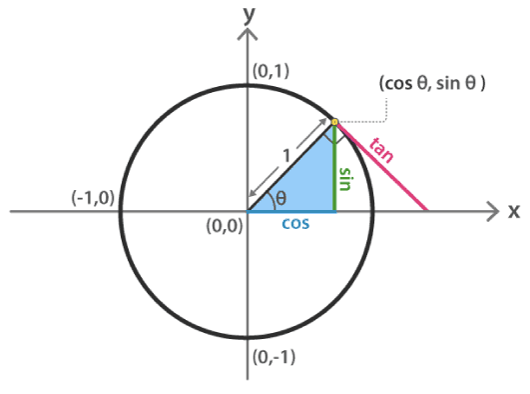
\includegraphics[width = .6\textwidth]{trigUnitCircle}
				\caption{Image of a trigonometric unit circle}
				\label{Fig:Trig Unit Circle}
			\end{figure}
		
		\subsection{Table of trigonometric values}
			{
				\centering
				\begin{tabular}{|c|c|c|c|c|c|c|c|c|}
					\hline \rowcolor{customOlive}
					$\alpha_{deg}$ & \degC{0} & \degC{30} & \degC{45} & \degC{60} & \degC{90} & \degC{180} & \degC{270} & \degC{360} \\ \hline
					$\alpha_{rad}$ & 0 & $\frac{\pi}{6}$ & $\frac{\pi}{4}$ & $\frac{\pi}{3}$ & $\frac{\pi}{2}$ & $\pi$ & $\frac{3\pi}{2}$ & $2\pi$ \\ \hline
					$\sin(\alpha)$ & 0 & $\frac{1}{2}$ & $\frac{1}{\sqrt{2}}$ & $\frac{\sqrt{3}}{2}$ & 1 & 0 & -1 & 0 \\ \hline
					$\cos(\alpha)$ & 1 & $\frac{\sqrt{3}}{2}$ & $\frac{1}{\sqrt{2}}$ & $\frac{1}{2}$  & 0 & -1 & 0 & 1 \\ \hline
					$\tan(\alpha)$ & 0 & $\frac{1}{\sqrt{3}}$ & 1 & $\sqrt{3}$ & \textcolor{red}{X} & 0 & \textcolor{red}{X} & 0 \\ \hline
				\end{tabular}
				\par
			}
		\pagebreak
	

		\subsection{Trigonometric Identities}
			\subsubsection{Trigonometry basis}
				\begin{itemize}
					\item $\tan(\theta) = \frac{\sin(\theta)}{\cos(\theta)}$
					\item $\cot(\theta) = \frac{\cos(\theta)}{\sin(\theta)}$
					\item $\tan(\theta) = \frac{1}{\cot(\theta)}$
					\item $\cot(\theta) = \frac{1}{\tan(\theta)}$
					\item $\sec(\theta) = \frac{1}{\cos(\theta)}$
					\item $\csc(\theta) = \frac{1}{\sin\theta)}$
				\end{itemize}
			\subsubsection{Pythagorean Identities}
				\begin{itemize}
					\item $\sin^2(\theta) + \cos^2(\theta) = 1$
					\item $\tan^2(\theta) + 1 = \sec^2(\theta)$
					\item $\cot^2(\theta) + 1 = \csc^2(\theta)$
				\end{itemize}

			\subsubsection{Reflections}
				\begin{itemize}
					\item $\sin(-\theta) = -\sin(\theta)$
					\item $\cos(-\theta) = \cos(\theta)$
					\item $\tan(-\theta) = -\tan(\theta)$
					\item $\cot(-\theta) = -\cot(\theta)$
					\item $\sec(-\theta) = \sec(\theta)$
					\item $\csc(-\theta) =  -\csc(\theta)$ 
				\end{itemize}

			\subsubsection{Angle Sum and Difference}
				\begin{itemize}
					\item $\sin(\alpha \pm \beta) = \sin(\alpha)\cos(\beta) \pm \sin(\beta)\cos(\alpha)$
					\item $\cos(\alpha \pm \beta) = \cos(\alpha)\cos(\beta) \mp \sin(\alpha)\sin(\beta)$
					\item $\tan(\alpha \pm \beta) = \frac{\tan(\alpha) \pm \tan(\beta)}{1 \mp \tan(\alpha)\tan(\beta)}$ 
					\item $\cot(\alpha \pm \beta) = \frac{\cot(\alpha)\cot(\beta) \mp 1}{\cot(\alpha) \pm \cot(\beta)}$
				\end{itemize}

			\subsubsection{Double Angle}
				\begin{itemize}
					\item $\sin(2\theta) = 2\sin(\theta)\cos(\theta)$
					\item $\cos(2\theta) = \cos^2(\theta) - \sin^2(\theta)$
					\item $\tan(2\theta) = \frac{2\tan(\theta)}{1-\tan^2(\theta)}$
					\item $\cot(2\theta) = \frac{\cot^2(\theta) - 1}{2\cot(\theta)}$
					\item $\sec(2\theta) = \frac{\sec^2(\theta)}{2-\sec^2(\theta)}$
					\item $\csc(2\theta) = \frac{\sec(\theta)csc(\theta)}{2}$
				\end{itemize}
			\subsubsection{Half Angle}
				\begin{itemize}
					\item $\sin(\frac{\theta}{2}) = \pm \sqrt{\frac{1-\cos(\theta)}{2}}$
					\item $\cos(\frac{\theta}{2}) = \pm  \sqrt{\frac{1+\cos(\theta)}{2}}$
					\item $\tan(\frac{\theta}{2}) = \frac{1-\cos(\theta)}{\sin(\theta)}$
				\end{itemize}	

		\subsection{Finding the 2nd solution}
			\noindent If we get asked to find for what values of x is $\sin(x)$ a value that is between -1 and 1 we know in the range from $0 \rightarrow 2\pi$ there are 2 answers. If sin(x) is given to us in the $1^{st}$ quadrant, then the second solution
			can be found 
				\[\sin(180^{\circ} - x)\]
			
			\noindent And if $\cos(x)$ is given in the same quadrant the second solution can be found by using this equation
				\[\cos(360^{\circ} - x)\]

			\hline \vspace{3mm}

			\noindent However if you want to find the negative solution but you only have the knows values for the positive values you can do the following. Find the x such that $\sin(x)$ is equal to the value you want to find (if you want to find
			$-\frac{1}{2}$ you will just take the value for x such that u get $sin(x) = \frac{1}{2}$). Afterwards you will use this equality to find your answer
				\[\sin(180^{\circ} + x) \lor \sin(360^{\circ} - x)\]

			\noindent And for $\cos(x)$ the equation is
				\[\cos(180^{\circ} \mp x)\]
	\section{Quadric Equations}
		\subsection{Introduction}
			\noindent Quadric equations are $2^{nd}$ degree polynomials meaning they have the form of:
			
			\begin{equation*}
				a*x^2 + b*x + c
			\end{equation*}

			\noindent Now that we got that out of the way lets talk about some important variables that decide how our parabola will end up looking.

			\subsubsection{Discriminant}
				\noindent The discriminant is defined in the following way:
				
				\begin{equation*}
					D = b^2 - 4*a*c
				\end{equation*}

				\noindent The discriminant together with the constant \emph{a} can tell us about how the function looks like.
			
		\subsection{Function Plots}
			\subsubsection{$D > 0 \land a > 0$}
				\begin{center}
					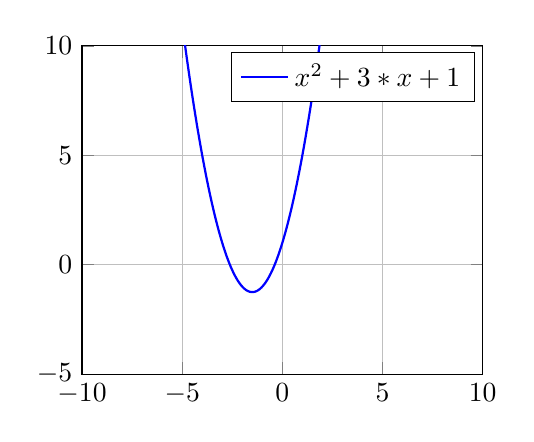
\begin{tikzpicture}
    						\begin{axis}[xmin = -10, xmax = 10, ymin = -5, ymax = 10,grid = both, major grid style = {lightgray}, minor grid style = {lightgray!25}, width = .55\textwidth] 
							\addplot[samples = 300, domain = -10:10, thick, smooth, blue]{x^2 + 3*x + 1};
							\legend{$x^2 + 3*x + 1$}
    						\end{axis}
					\end{tikzpicture}
				\end{center}
				\noindent We can say that the function will have 2 points ($x_{1,2}$) where it's value will be 0 ($y = f(x) \implies y = 0 = f(x_{1,2})$). We can also see that between points $x_1$ and $x_2$ the function is negative and everywhere else it
				is positive. So we can confirm the following:

				\begin{itemize}	
					\item $f(x) < 0 \rightarrow x \in (x_1, x_2)$
					\item $f(x) > \rightarrow  x \in (-\infty, x_1) \bigcup (x_2, +\infty)$
					\item $f(x) = 0 \rightarrow x = x_{1,2}$
				\end{itemize}	

				\pagebreak

			\subsubsection{$D > 0 \land a < 0$}	
				\begin{center}
					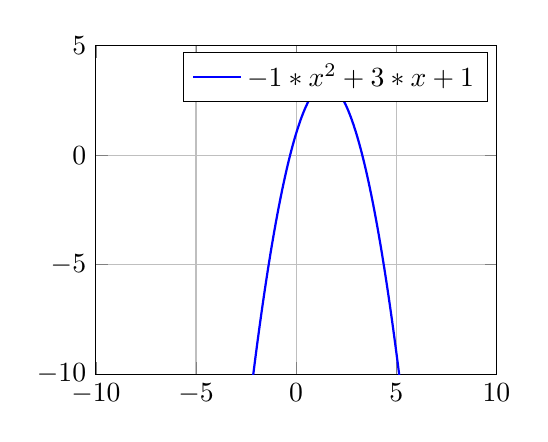
\begin{tikzpicture}
    						\begin{axis}[xmin = -10, xmax = 10, ymin = -10, ymax = 5,grid = both, major grid style = {lightgray}, minor grid style = {lightgray!25}, width = .55\textwidth] 
							\addplot[samples = 300, domain = -10:10, thick, smooth, blue]{-1*x^2 + 3*x + 1};
							\legend{$-1*x^2 + 3*x + 1$}
    						\end{axis}
					\end{tikzpicture}
				\end{center}
				
				\begin{itemize}	
					\item $f(x) > 0 \rightarrow x \in (x_1, x_2)$
					\item $f(x) < 0 \rightarrow  x \in (-\infty, x_1) \bigcup (x_2, +\infty)$
					\item $f(x) = 0 \rightarrow x = x_{1,2}$
				\end{itemize}	

				
			\subsubsection{$D = 0 \land a > 0$}

				\begin{center}
					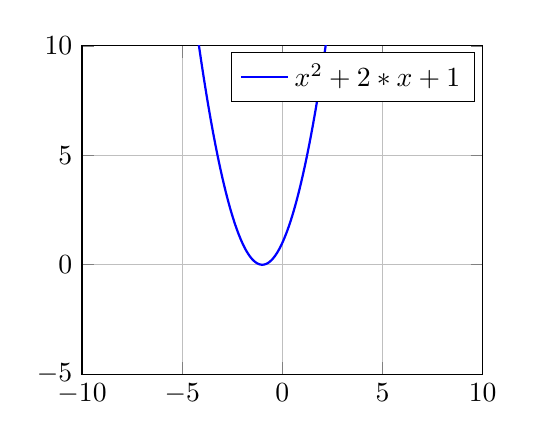
\begin{tikzpicture}
    						\begin{axis}[xmin = -10, xmax = 10, ymin = -5, ymax = 10,grid = both, major grid style = {lightgray}, minor grid style = {lightgray!25}, width = .55\textwidth] 
							\addplot[samples = 300, domain = -10:10, thick, smooth, blue]{x^2 + 2*x + 1};
							\legend{$x^2 + 2*x + 1$}
    						\end{axis}
					\end{tikzpicture}
				\end{center}

				\noindent Here we can see that when $D = 0$ there is only \emph{one x} for which $y = 0$ and we will call this x $x_1$, and for positive values of a this function is never negative

				\begin{itemize}	
					\item $f(x) < 0 \rightarrow x \in \emptyset$
					\item $f(x) > 0 \rightarrow  x \in (-\infty, x_1) \bigcup (x_1, +\infty)$
					\item $f(x) = 0 \rightarrow x = x_{1}$
				\end{itemize}	
				\pagebreak

			\subsubsection{$D = 0 \land a < 0$}
				
				\begin{center}
					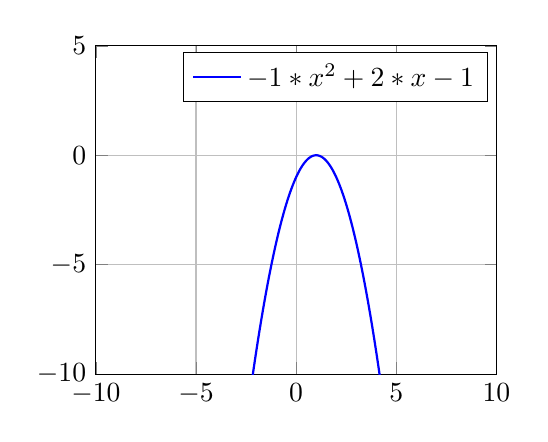
\begin{tikzpicture}
    						\begin{axis}[xmin = -10, xmax = 10, ymin = -10, ymax = 5,grid = both, major grid style = {lightgray}, minor grid style = {lightgray!25}, width = .55\textwidth] 
							\addplot[samples = 300, domain = -10:10, thick, smooth, blue]{-1*x^2 + 2*x - 1};
							\legend{$-1*x^2 + 2*x - 1$}
    						\end{axis}
					\end{tikzpicture}
				\end{center}

				\begin{itemize}	
					\item $f(x) > 0 \rightarrow x \in \emptyset$
					\item $f(x) < 0 \rightarrow  x \in (-\infty, x_1) \bigcup (x_1, +\infty)$
					\item $f(x) = 0 \rightarrow x = x_{1}$
				\end{itemize}	
			\subsubsection{$D < 0 \land a > 0$}
				
				\begin{center}
					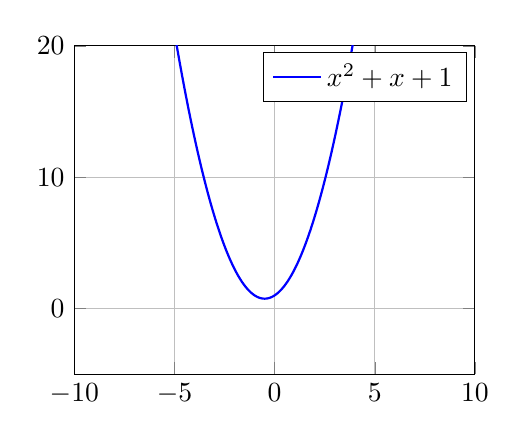
\begin{tikzpicture}
    						\begin{axis}[xmin = -10, xmax = 10, ymin = -5, ymax = 20,grid = both, major grid style = {lightgray}, minor grid style = {lightgray!25}, width = .55\textwidth] 
							\addplot[samples = 300, domain = -10:10, thick, smooth, blue]{x^2 + x + 1};
							\legend{$x^2 + x + 1$}
    						\end{axis}
					\end{tikzpicture}

					\noindent In this case we can see that the function is always positive for every values of x.

				\end{center}
				
				\begin{itemize}	
					\item $f(x) > 0 \rightarrow x \in (-\infty, +\infty)$
					\item $f(x) < 0 \rightarrow  x \in \emptyset$ 
					\item $f(x) = 0 \rightarrow x \in \emptyset$
				\end{itemize}
				\pagebreak

			\subsubsection{$D < 0 \land a < 0$}
				
				\begin{center}
					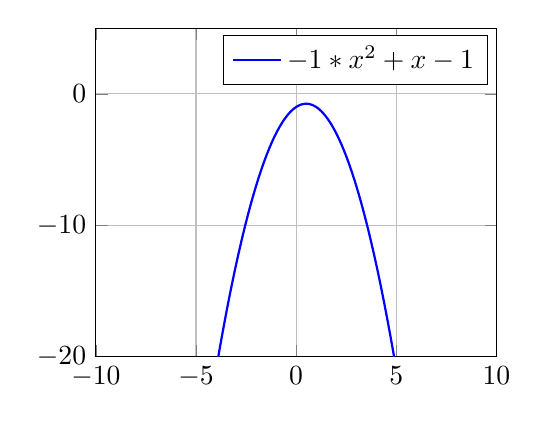
\begin{tikzpicture}
    						\begin{axis}[xmin = -10, xmax = 10, ymin = -20, ymax = 5,grid = both, major grid style = {lightgray}, minor grid style = {lightgray!25}, width = .55\textwidth] 
							\addplot[samples = 300, domain = -10:10, thick, smooth, blue]{-1*x^2 + x - 1};
							\legend{$-1*x^2 + x - 1$}
    						\end{axis}
					\end{tikzpicture}
				\end{center}

				\begin{itemize}	
					\item $f(x) > 0 \rightarrow x \in \emptyset$
					\item $f(x) < 0 \rightarrow x \in (-\infty, +\infty)$
					\item $f(x) = 0 \rightarrow x \in \emptyset$
				\end{itemize}

		\subsection{Finding zero points}
			\noindent To find the values for x for which $y = 0$ we will simply apply the following formula:
			\begin{equation*}
				x_{1,2} = \frac{-b \pm \sqrt{D}}{2a} = \frac{-b \pm \sqrt{b^2 - 4ac}}{2a} 
			\end{equation*}

	\section{Equation of lines}
		\subsection{Introduction}
			\noindent When we talk about straight lines there are 2 ways we describe them.
			\begin{enumerate}
				\item $y = kx + n$
				\item $y = y_0 + k(x - x_0)$
			\end{enumerate}

			\noindent $k$ is the slope of the line and can be calculated by taking the difference of change over y with respect to x.
			\begin{equation}
				k = \frac{f(x_2) - f(x_1)}{x_2 - x_1} = \frac{\bigtriangledown y}{\bigtriangledown x}
			\end{equation}

			\noindent $n$ is the Y intercept and it tells us where does the line touch the y axis when $x = 0$ \\
			\noindent For the 2nd equation $y_0$ is just the y value of a starting points and $x_0$ is the x value of some starting point that we took. Everything else is the same.
		
			\subsubsection{example}
				
				\begin{center}
					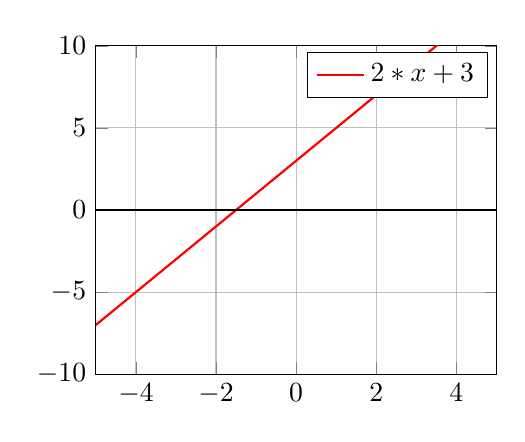
\begin{tikzpicture}
    						\begin{axis}[xmin = -5, xmax = 5, ymin = -10, ymax = 10,grid = both, major grid style = {lightgray}, minor grid style = {lightgray!25}, width = .55\textwidth] 
							\addplot[samples = 300, domain = -10:10, thick, smooth, red]{2*x + 3};
							\addplot[samples = 300, domain = -10:10, thick, smooth, black]{0};
							\legend{$2*x + 3$}
    						\end{axis}
					\end{tikzpicture}
				\end{center}

				\noindent As we can see from the equation $y = 2*x + 3$ we can tell that our $n = 3$ and our $k = 2$ this means at $x = 0$ the line will touch the y axis at point $A(0,3)$ and for every change in x y doubles, so if x goes from
				$0 \rightarrow 2$ y will go from $0 + n \rightarrow 4 + n$
		\subsection{Conditions for paralel lines}
			\noindent If two lines are paralel that means that their slope $k$ is the same (A.K.A $k_1 = k_2$)

			\begin{center}
				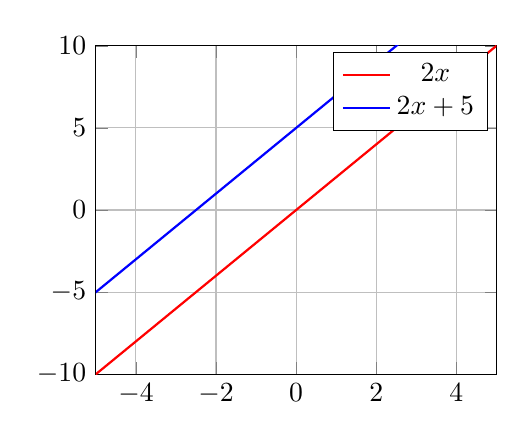
\begin{tikzpicture}
    					\begin{axis}[xmin = -5, xmax = 5, ymin = -10, ymax = 10,grid = both, major grid style = {lightgray}, minor grid style = {lightgray!25}, width = .55\textwidth] 
						\addplot[samples = 300, domain = -10:10, thick, smooth, red]{2*x};
						\addplot[samples = 300, domain = -10:10, thick, smooth, blue]{2*x + 5};
						\legend{$2x$,$2x + 5$}
    					\end{axis}
				\end{tikzpicture}
			\end{center}

			\pagebreak
		\subsection{Conditions for perpendicular lines}
			\noindent For two lines to be perpendicular their slopes must be negative inverses of one another (A.K.A $k_1 = -\frac{1}{k_2}$)
			
			\begin{center}
				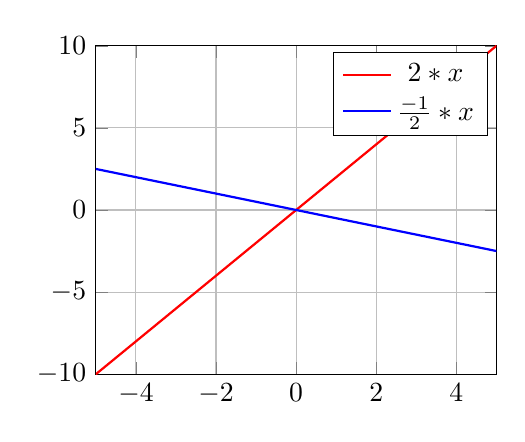
\begin{tikzpicture}
    					\begin{axis}[xmin = -5, xmax = 5, ymin = -10, ymax = 10,grid = both, major grid style = {lightgray}, minor grid style = {lightgray!25}, width = .55\textwidth] 
						\addplot[samples = 300, domain = -10:10, thick, smooth, red]{2*x};
						\addplot[samples = 300, domain = -10:10, thick, smooth, blue]{-x/2};
						\legend{$2*x$, $\frac{-1}{2}*x$}
    					\end{axis}
				\end{tikzpicture}
			\end{center}
	\section {Equation of a circle}
		\subsection{Introduction}
			\noindent To understand this part we better take a look at what a circle actually is. By definition a circle is a group of points that have the same distance from once center points; meaning that we will first have to take a look at the equation
			of distance. The equation of distance between two points goes as follows.

			\begin{equation*}
				d = \sqrt{(x_1 - x_2)^2 + (y_1 - y_2)^2}
			\end{equation*}

			\noindent If we take $x_2$ and $y_2$ to be the cordinants of the center of the circle and write them as $x_c$ and $y_c$, and if we take $r$ to be the radius we will get the following equation.
			
			\begin{equation*}
				r = \sqrt{(x_1 - x_c)^2 + (y_1 - y_c)^2}
			\end{equation*}

			\noindent If the center of the circle is at the center of the cordinate system (0,0) then we get the equation.
			
			\begin{equation*}
				r = \sqrt{x^2 + y^2} \implies r^2 = x^2 + y^2
			\end{equation*}

			\noindent Where $x$ and $y$ are points in the cordinate system.
	
		\pagebreak
		\subsection{Problem solving}
			\noindent If we have a question that asks us to find a circle that fits points A and B we have to find a point C such that the distance $\overline{AC}$ must be the same as the distance $\overline{BC}$. To do this we can just find the distance
			$\overline{AB}$ and divide it by 2 to get our radius, but this will lead us to a complicated way to find the solution; so we will find the point in between A and B. To find a point that is between two other points it is as simple as solving the
			following set of equations.

			\begin{equation*}
				A(x_1, y_1)
			\end{equation*}
			
			\begin{equation*}
				B(x_2, y_2)
			\end{equation*}
			
			\begin{equation*}
				C(\frac{x_1 + x_2}{2}, \frac{y_1 + y_2}{2})
			\end{equation*}

			\begin{center}
				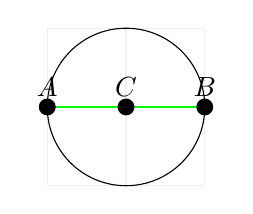
\begin{tikzpicture}
					\draw[lightgray!25] (-1,-1) grid (1,1);
					\draw (0,0) circle (1);
					\draw node at (0,.25) {$C$};
					\draw node at (-1,.25) {$A$};
					\draw node at (1,.25) {$B$};
					\draw[green] (-1,0) -- (1,0);
					\filldraw (0,0) circle (1mm);
					\filldraw (1,0) circle (1mm);
					\filldraw (-1,0) circle (1mm);
				\end{tikzpicture}
			\end{center}
			
			\hline \vspace{3mm}
			\noindent Another type of problem is when you are given the center of the circle and it's radius and you are suppose to find out if a given point belongs to the circle, but this is simple just plug it into the equation given beforehand and see
			if the distance between the center and the given point is the same as the radius.
			
\end{document}
